\newpage
\section{The Mu2e DAQ system}
\label{sec:daq}
The Mu2e Trigger and Data Acquisition (DAQ) subsystem collectd, filters, and  monitors the digitized data from the differnt sub-detectors; delivers the data to online and offline processing for analysis; and  synchronizes and controls the detector readout. The DAQ system is based on a “streaming” readout in which all detector data are digitized and zero-suppressed in detector front-end electronics before being transmitted to the DAQ system. While this approach results in a larger data rate, it provides a simpler architecture with a greater flexibility in data filtering and monitoring. The DAQ system uses otsdaq\cite{} as a solution, togeether with the artdaq~\cite{} and art~\cite{} framework to process and filter events. 

An overview of the full system is shown in Figure~\ref{fig:daqoverview}, displaying the following components:

\begin{itemize} 
\item The Readout Controllers (ROC) are reading out, digitizing and streaming the data from the readout electronics to the DTC. There are 216 ROCs for the tracker, 140 ROCs for the calorimeter, 16 ROCS for the CRV, 1 ROC for the ExtMon and 1 ROC for the STM. The data, timing signal and detector control signals are transmitted over a single link from the DTC to tracker / calorimeter ROCs. The timing signal is transported in a separate link for the CRV, while the data are transmitted via ethernet for the monitors. 

\item The Data Transfer Controller (DTC) receives the system clock and event readout request from the CFO and timing fanout module, and reads out data from the ROC. They are installed in the DAQ servers - up to 2 DTCs per a server - and are connected to a maximum of 6 ROCs. Each tracker/calorimeter DTC receives the data of a fraction of the detector, and the data are shuffled among the DTCs via Event Building Switches to form a complete event. The data from the CRV are only pulled for requested (triggered) events. 

\item The Command fanout module (CFO) is responsible for generating and synchronizing readout requests. It receives the accelerator zero-crossing marker, supplies a continuous clock to the DTCs and sends readout requests control packets for each system clock. A timing fanout module is used to broadcast the system clock to drive the transmit link in chain of DTCs to prevent jitter accumulation

\item The DAQ servers contain the DTCs and run the online trigger software. The DTCs in each server are connected to two different event building networks. Triggered events are sent to the data logger node, and a dispatcher forwards in a non-blocking way a subset of events to the data quality monitoring nodes. Slow control monitoring (EPICS) runs on the EPICS host. Communication is performed over two networks: the DCS \& management network and the control \& data storage network. Communication to the lab network is managed by gateway nodes. 
\end{itemize} 
intensity variations via luminosity streams. These proxies include, among others, the total number of reconstructed proton candidates or the total energy deposited in the calorimeter. A dedicated debug stream is also used to further analyze events producing exceptions in the algorithm chains.  

\begin{figure}[htb]
\begin{center}
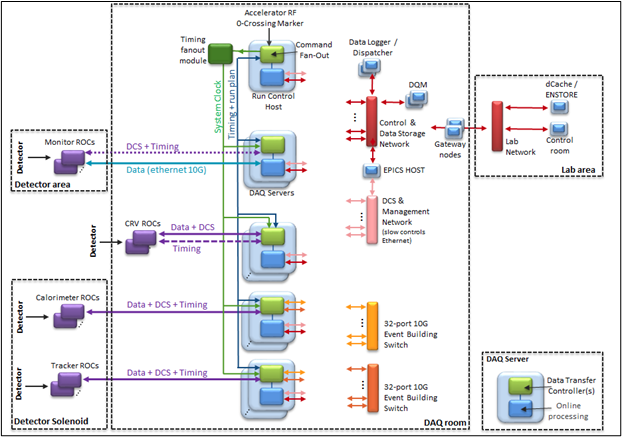
\includegraphics[width=0.9\linewidth]{figures/daq-overview.png}
\caption{Overview of the Mu2e DAQ system}
\label{fig:daqoverview}
\end{center}
\end{figure}

The data flow starts with the tracker and calorimeter DTCs forwaring readout requests from the CFO to their ROCs. The ROCs read out the detector data in response and the DTC collects ROC data for a given Event Window Tag (EWT, a unique tag sent by the CFO to define an event). Each DTC stores a fraction of the detector data in its memory. The DTCs are grouped into two sets, connected among themselves via an event building network (in a given server, each DTC is connected to a different network). In each group of DTCs, one DTC acts as an Event Builder for a given EWT, and the remaining DTCs send their data to that DTC via the event building network. The system is set such that the two halves of an event are built by two DTCs in the same server. The two halves of an event are transferred from the DTCs to the main memory by an ArtdaqBoardReader process, which creates fragments and sends them to the ArtdaqEventBuilder process. The ArtdaqEventBuilder runs the online trigger software on the tracker and calorimeter data. In addition, information from the intensity streams are sent to a data logger. Triggered events are forwarded to a secondary ArtdaqEventBuilder. Information from the CRV is requested via an ArtdaqBoardReader process. The BoardReader instructs the DTC to fetch the corresponding EWT data from the CRV ROCs. A fully assembled event is finally forwarded to a data logger node to be persisted to disk. A dispatcher sends a subset of events in a non-blocking way to the data quality monitoring (DQM) nodes. The dispatcher cannot interrupt data logging, events are simply not forwarded if the DQM nodes are all busy. The DQM metrics are periodically forwarded to the online monitoring nodes.

Physics and calibration data are selected by a set of filtering algorithms organized into a series of streams. Each stream combines algorithms to identify a well-defined event topology (e.g. a track with a momentum greater than a certain threshold or a high energy cluster in the calorimeter). The artdaq architecture can re-use the output of a given algorithm if it appears in multiple streams, thus minimizing the running time of the online processing. Prescaled factors can be adjusted for each stream independently to tune the total trigger rate. Similarly, streams can be enabled or disabled depending on the beam conditions (on-spill or off-spill).   

The trigger filters must provide a signal efficiency larger than 90\%, reduce the average data rate by a factor of 400 or more, and achieve a processing time of less than 5 ms/event. The main physics triggers is based on information from reconstructed tracks and, to some extend, reconstructed calorimeter clusters. The track reconstruction algorithms is factorized into three main parts:
\begin{itemize}
\item Hits reconstruction from the digitized signals recorded by the tracker. Each signal is transformed into a hit along the tracker wires. A multivariate classifier is used to reject hits produced by a low-momentum Compton electron 
\item Pattern-recognition to select group of hits compatible with helicoidal trajectories. Two separate methods are used: a calorimeter-seeded and a tracker-seeded algorithm;
\item Track fit to increase the accuracy of the reconstructed track and improve the background rejection. A simplified Kalman fit is finally performed to improve the accuracy of the 
reconstructed track parameters and further reject spurious candidates.
\end{itemize}

The resulting efficiency for conversion electrons is around 98\% for the nominal proton bunch intensity, with a background rejection factor greater than 1000, and the efficiency only decreases by a few percents for proton bunch intensity up to three times the nominal value. Other trigger streams include, for example, $\mu^- \rightarrow e^+$ conversion electrons, high-momentum decay-in-orbit electrons, high energy photons produced by radiative pion or muon capture, cosmic rays, or electrons from muons stopping in the internal proton absorber.

In addition, summary information are saved for every micro-bunch to estimate instantaneous proton intensity variations via luminosity streams. These proxies include, among others, the total number of reconstructed proton candidates or the total energy deposited in the calorimeter. A dedicated debug stream is also used to further analyze events producing exceptions in the algorithm chains.  